
\documentclass{article}

\usepackage[utf8]{inputenc}
\usepackage{graphicx}

\usepackage{tikz}

\usepackage[headheight = 2.98cm, includehead, margin = 1cm ]{geometry}
\pagestyle{empty}


\newdimen\odsLogoWidth
\odsLogoWidth35mm\relax

% First letter of logo has a width of ca. 21/94 of the total logo width 
% This amount of white space should be used on both sides of the logo
\newdimen\odsOWidth 
\odsOWidth\dimexpr\dimexpr\odsLogoWidth*21\relax/94\relax


\def\numdivisions#1#2#3{%
    \newcount\divs%
    \divs\numexpr#2/\dimexpr#3\relax\relax%
    % TeX rounds result of division to nearest integer
    % We want floor division, so we advance the result by -1 if it was rounded up
    \ifnum\numexpr\divs*\dimexpr#3\relax\relax>\numexpr#2\relax\advance\divs by -1\fi%
    #1\divs\relax%
}

% Vertical rule of height \vsize and width #1
% Has negative whitespace on the left and right equal to #1/2
\def\centvrule#1{\def\hds{\hskip\dimexpr-#1/2\relax}\hds\rule{#1}{\vsize}\hds\relax}

\begin{document}


\newcount\hdivs
\newcount\vdivs

\numdivisions{\vdivs}{\textheight}{1cm}
\numdivisions{\hdivs}{\textwidth}{1cm}

\newdimen\vrulewidth
\vrulewidth .4pt\relax

%\advance\vdivs by -1

\makeatletter

% Define header
% #1 : dimension of available space
\def\ods@head#1{%
% Calculate available space
\newdimen\availableHSize%
\availableHSize#1%
% Set width of end section
\newdimen\endSection%
\endSection 4cm\relax%
% Calculate width of mid section
\newdimen\midSection%
\expandafter\midSection\dimexpr\availableHSize - \odsLogoWidth - \odsOWidth - \endSection\relax%
%
\noindent\hbox to \hsize{\vsize\headheight\relax%
    \parskip 0pt\relax%
    \baselineskip 0pt\relax%
    \noindent\hfill%
    
\includegraphics[width=\odsLogoWidth]{odslogo.jpg}%
    \hskip\dimexpr\odsOWidth/2\relax\relax%
    \centvrule{\vrulewidth}%
    \hskip\dimexpr\odsOWidth/2\relax\relax%
    \vbox to \vsize{\hsize\midSection\relax%
        {\large\bfseries \textgreater generic graph paper}\par%
        \vfil%
        {\sc\large Name: \leaders\hrule\hfill\hbox{}}\par%
        \vskip3ex\relax%
        {\sc\large Project: \leaders\hrule\hfill\hbox{ }}\par%
        \vskip3ex\relax%
        {\sc\large Title: \leaders\hrule\hfill\hbox{ }}%
    }%
    \vbox to \vsize{\hsize\endSection\relax%
        \vfill%
        {\large\sc\rule{0pt}{0pt}\leaders\hrule\hfill\hbox{}}\par%
        \vskip3ex\relax%
        {\sc\large Date: \leaders\hrule\hfill\hbox{ }- \leaders\hrule\hfill\hbox{ }- \leaders\hrule\hfill\hbox{}}\par%
        \vskip3ex\relax%
        {\sc\large Page: \leaders\hrule\hfill\hbox{ }of \leaders\hrule\hfill\hbox{}}\par%
    }%
    \hfill%
}%
}
\newdimen\cmm 
\cmm 1cm\relax
\multiply\cmm by 19

\def\@oddhead{\ods@head{\cmm}}
\makeatother




% Make sure there is a nondiscardable on first line, and there is no extra white space
\topskip 0pt\vbox to 0pt{}%
%
% Center vertically 
\vfill%
% 
% Make sure there is no unwanted white space and center horizontally
\noindent\hfil%
%
% Draw the grid 
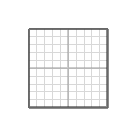
\begin{tikzpicture}[x=1cm, y=1cm, semitransparent]
\draw[step=1mm, line width=0.1mm, black!30!white] (0,0) grid (\hdivs,\vdivs);
\draw[step=5mm, line width=0.2mm, black!40!white] (0,0) grid (\hdivs,\vdivs);
\draw[step=1cm, line width=0.3mm, black!90!white] (0,0) grid (\hdivs,\vdivs);
\end{tikzpicture}%
%
% Center horizontally and vertically, end page
\hfil\vfill\relax\eject


\end{document}